% 2011 年湖南卷理科第 15 题：圆内接正方形与扇形 OHE。
% 来源 PDF：普通高考/2011/2011湖南理.pdf，SHA-256 09b67f1db8e6a280165cf8431211a968163c0d0f262a50068dd607607a9ec578。
% 原页：第 1 页第 3 栏中部，书页码 671。
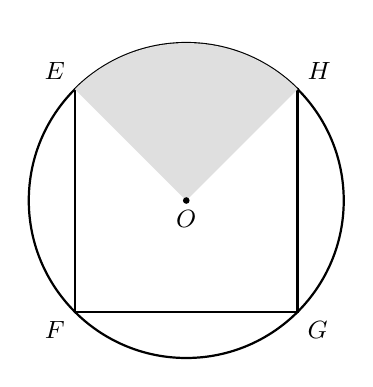
\begin{tikzpicture}[>=stealth, semithick, font=\small, scale=1.0]
  \draw[thick] (0,0) circle (2);
  \coordinate (E) at (-1.414,1.414);
  \coordinate (H) at (1.414,1.414);
  \coordinate (F) at (-1.414,-1.414);
  \coordinate (G) at (1.414,-1.414);
  \draw[thick] (E)--(H)--(G)--(F)--cycle;
  \fill[gray!25] (0,0)--(H) arc (45:135:2)--cycle;
  \fill (0,0) circle (1.2pt) node[below] {$O$};
  \node[above left] at (E) {$E$};
  \node[above right] at (H) {$H$};
  \node[below left] at (F) {$F$};
  \node[below right] at (G) {$G$};
\end{tikzpicture}
